\section{Theoretical and technical background}
\subsection{Basics of Nuclear Magnetic Resonance}

Nuclear Magnetic Resonance techniques relay of the interaction between the magnetic dipole moment
\begin{equation}
\label{magnetic dipole moment}
\vec{\mu} = \hbar\gamma\vec{S} 
\end{equation}
 of nuclei with non-zero spin $S$ and an external magnetic field $\vec{B_0}$. Here $\gamma$ represents the gyro-magnetic ratio of protons:
$$ \gamma_{proton} = 2.6752 \cdot 10^8 \, \textrm{sec}^{-1}\textrm{Tesla}^{-1}.
$$The resulting interaction energy, also called spin-lattice contribution, is defines as:
\begin{equation}
\label{interaction energy}
\Delta E = -\vec{\mu}\cdot\vec{B}_0.
\end{equation}

This interaction yields two states for the orientation of the protons' magnetic dipole in the external magnetic field: $\mu_+$ (parallel) and $\mu_-$ (anti-parallel).
For a macroscopic sample of $N$ protons, both numbers of occupied states $N_+$ and $N_-$, the sum of which comprises $N$, can be approximated by a Boltzmann distribution.
%:
%\begin{equation}
%\label{ocupation number}
% N_\pm = N_0e^{-\frac{E_0\pm\Delta E}{kt}}
%\end{equation}
%with $N_0$ as a normalization factor. 
Due to the parallel state being energetically favorable, one observes $N_+>N_-$. The predominance of protons in the parallel state leads to a macroscopic magnetization.
% whose ground state is
%\begin{equation}
%\label{magnetization ground state}
%\vec{M}_0 = \frac{\mu N}{V}\sinh{\left(\frac{\mu B}{kT}\right)} \vec{e}_z .
%\end{equation}
In our case, of a weak field ($\mu B \gg kT$), the ground state of the system can be approximated by:
\begin{equation}
\label{ground state approx}
\vec{M}_0 = \frac{N}{V} \frac{\hbar^2 \gamma^2 I(I+1)}{3kT}\vec{B}_0 \propto \frac{\vec{B}_0}{T},
\end{equation}
i.e the law of Curie.

In general, the magnetization can have an arbitrary orientation related to the external magnetic field, however such a system will decay asymptotically into the ground state, since $\vec{M}_0$ minimizes the energy. 

The interaction between the macroscopic magnetization and the external magnetic field result in a torque:
\begin{equation}
\vec{\tau} = \gamma\vec{M} \wedge\vec{B}_0.
\end{equation}
If the magnetization is separated into parallel $\vec{M}_{\parallel}$ and perpendicular $\vec{M}_{\perp}$ components, relative to the external field, we  see that only the later gives a non-trivial expression. Without any relaxation processes, the rate of change of the former is given by:
\begin{equation}
\frac{d \vec{M}_{\perp}}{dt} = -\vec{M}_{\perp}\wedge\vec{B}_0.
\end{equation}
The last equation describes the precession of $\vec{M}_{\perp}$ around $\vec{B}_0$. The angular frequency of this process is called the Larmor frequency:
\begin{equation}
\label{eq: larmor freq}
\omega_L = \gamma B_0.
\end{equation}

Generating a transverse or anti-parallel magnetization to $\vec{B}_0$ can be achieved by applying a high frequency pulse to the ground state magnetization $\vec{M}_0$. 

For a static magnetic field $\vec{B}_0$ pointing in the z-direction, and a coil oriented along the x-axis, applying a sinusoidal voltage with a frequency $\omega_H$, would generate a solenoid magnetic field $\vec{B}_1$ polarized along the x-direction. Under this conditions the torque  acquires a second term:
\begin{equation}
\vec{\tau} = \vec{M}_0\wedge(\vec{B}_0 + \vec{B}_1(t)
\end{equation}
which induces a second precession around the x-axis.
For a pulse duration, which is short relative to the relaxation time, the magnitude of the magnetization is approximately constant. In this case the vector $\vec{M}$ moves in a sphere with radius $|\vec{M}_0|$. The vector coordinates in the sphere are then given by a azimuthal angle $\varphi$, which is defined by the precession induced by $\vec{B}_0$, and by a polar angle $\theta$ which arises from the interaction with the solenoid field. Both angles are a functions of time:
\begin{equation}
\varphi = \omega_L t
\end{equation}
\begin{equation}
\theta = \gamma B_1 t.
\end{equation}

A pulse which induces a  polar angle $\theta = 90$° is called a 90° pulse. For such a pulse the ground state magnetization is transformed into transverse magnetization $\vec{M}_{\perp}$%, with $\vec{M}_{\parallel} = 0$
. Analogously a pulse which generates $\theta = 180°$ is called a 180° pulse. Such a pulse transforms the ground state into an anti-parallel magnetization $\vec{M}_{\perp} = -\vec{M}_0$. %, with $\vec{M}_{\parallel} = 0$.
\subsection{NMR signal}
\subsubsection{Signal generation}
In the set up used for this experiment, the high frequency pulses of fixed frequency $\omega_{HF} = 19.8$ MHz were generated in an electronic unit of the minispec p20. Said pulses induce a precession around the z-axis, that change the magnetic flux through the coil in time, resulting in a induction signal modulating by the Larmor frequency $\omega_L$, which could be set up by hand. This signal is fed back to the p20 electronic unit, where both the high frequency and the induction signals are mixed into an output given by the multiplication of both inputs, i.g the sum of two cosine functions. One of the terms depends on the working frequency, which is given by the difference between $\omega_L$ and $\omega_{HF}$, and is on the order of few hundred Hertz, while the second one in the range of 40MHz. The use of a low frequency bandpass filter allows to get rid of the former signal.   
\subsection{Relaxation Time}
\subsubsection{Bloch equations}
For the description of the precession of $\vec{M}_{\perp}$ it is possible to define a rotating reference system $(x', y', z)$. This reference frame is defined by 2 condition: 1) the $(x', y')$-plane rotate in the static $(x, y)$-plane and 2) $\vec{M}_{\perp}$ points in the $x'$-direction.

In this reference system the transverse and longitudinal magnetization are constant if no relaxations processes are present, otherwise both components are time dependent. Their time evolution is described by the Bloch equations:
\begin{equation}
\label{eq: bloch T2}
\frac{d\vec{M}_\perp^{rot}}{dt} = -\frac{\vec{M}_\perp^{rot}}{T_2}
\end{equation}
\begin{equation}
\label{eq: bloch T3}
\frac{d\vec{M}_\parallel^{rot}}{dt} = -\frac{\vec{M}_\parallel^{rot} - \vec{M}^{rot}}{T_1}.
\end{equation}
%In the later equations it is assumed that the time evolution is dominated by a restoring force which is linearly proportional to the deflection from equilibrium. 
The constant $T_2$ in eq. \ref{eq: bloch T2} is the so called spin-spin relaxation time, whereas $T_1$ in eq. \ref{eq: bloch T3} is called the spin-lattice relaxation time. The ground state is equal in the rotating and the static reference frame. 

In the presence of a relaxation processes, the time evolution of the magnetization in a laboratory $\vec{M}$ and in a rotating system $\vec{M}^{rot}$ are related :
%by 
%\begin{equation}
% \frac{d \vec{M}}{dt} = \frac{\partial \vec{M}^{rot}}{\partial t} + \vec{\omega}\wedge\vec{M}
% \end{equation}
 giving the following Bloch equations in laboratory system:
 \begin{equation}
 \label{bloch + rot T2}
   \frac{d \vec{M}_{\perp}(t)}{dt} = \gamma(\vec{B}\wedge\vec{M})_\perp - \frac{\vec{M}_\perp (T)}{T_2},
  \end{equation} 
  \begin{equation}
  \label{bloch + rot T1}
     \frac{d \vec{M}_{\parallel}(t)}{dt} = \gamma(\vec{B}\wedge\vec{M})_\parallel  -\frac{\vec{M}_\parallel (t)-\vec{M}_0}{T_1}.
  \end{equation}
 \subsubsection{Spin-spin relaxation $T_2$}
%The magnetic field that interacts with the magnetization is not constant, firstly due to possible variations of the applied static field, but more important due to 
Due to the magnetic interactions between the sample's protons with themselves, along with other phenomena, slowly varying field inhomogeneities are generated that cause
% Furthermore, thermally induced rotations as well as translations of nuclei, caused by molecular diffusion, throughout spatially varying magnetic environments will causes the field that any nucleus experiences to be time-dependent. 
the protons at different positions to precess with different frequencies. Hence a dephasing of the microscopic magnetizations takes place, i.e $\vec{M}_\perp$ decays to zero. This process is called spin-spin relaxation and it's characterized by the $T_2$ time. Said decay is described by the solution of eq. \ref{bloch + rot T2}:
\begin{equation}
\label{eq: sol. bloch T2}
\vec{M}_{\perp}(t)= \vec{M}_\perp^{0}e^{-\frac{t}{T_2}}.
\end{equation}
In the following experiment two different methods were used to measure $T_2$: 1) spin-echo/ Hahn echo method and 2) Carr-Purcell sequence. In both cases a 180° pulse is used to reverse the dephasing. 
\paragraph{Spin-Echo:}
The spin echo method consist on a 90° pulse that creates a transverse magnetization followed by a 180° pulse at $t = \tau$ that reverts the dephasing. One could imagine exchanging the position of protons that presses faster with the
% TODO: not sure about the wording
 slow ones.  After the pulse, all particles keep on rotating clockwise, such that at $t = 2\tau$ the fast protons catch up with the slow ones generating a spin-echo. The process is illustrated in Fig. \ref{fig: spin-echo}. 
\begin{figure}[!htbp]
 \begin{center}
  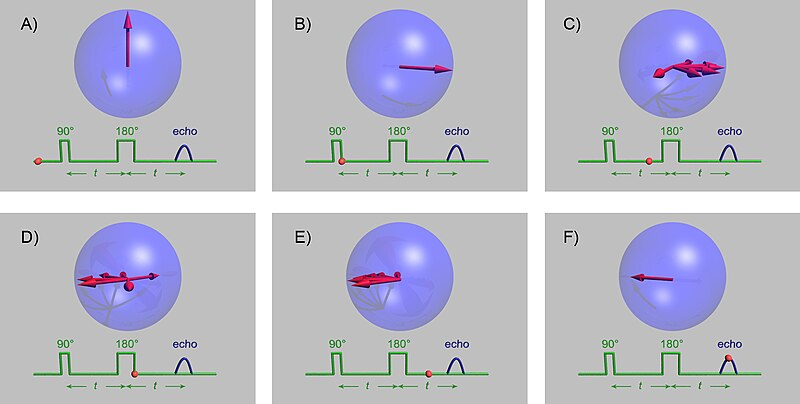
\includegraphics[width = .6\textwidth]{Latex images/SpinEcho_GWM_stills.jpg}
  \caption[]{Spin-echo method. a) system in ground state, b) 90° pulse, c) dephasing, c) 180° pulse, d) rephasing, e) coherence/ spin-echo  \footnotemark}
    \label{fig: spin-echo}
 \end{center}
\end{figure}
\footnotetext{Nuclear magnetic resonance. (2024, May 16). \href{Wikipedia. https://en.wikipedia.org&/wiki/Nuclear_magnetic_resonance}{Quelle: wikipedia.org}}
%The resulting signal is represented in Fig. \ref{fig: spin-echo signal}. There the decay of $\vec{M}_\perp$ is visible at time $t<5$ ms and the spin echo is to be seeing in the time range $15$ ms $< t < 25$ ms.
%\begin{figure}[!htbp]
% \begin{center}
%  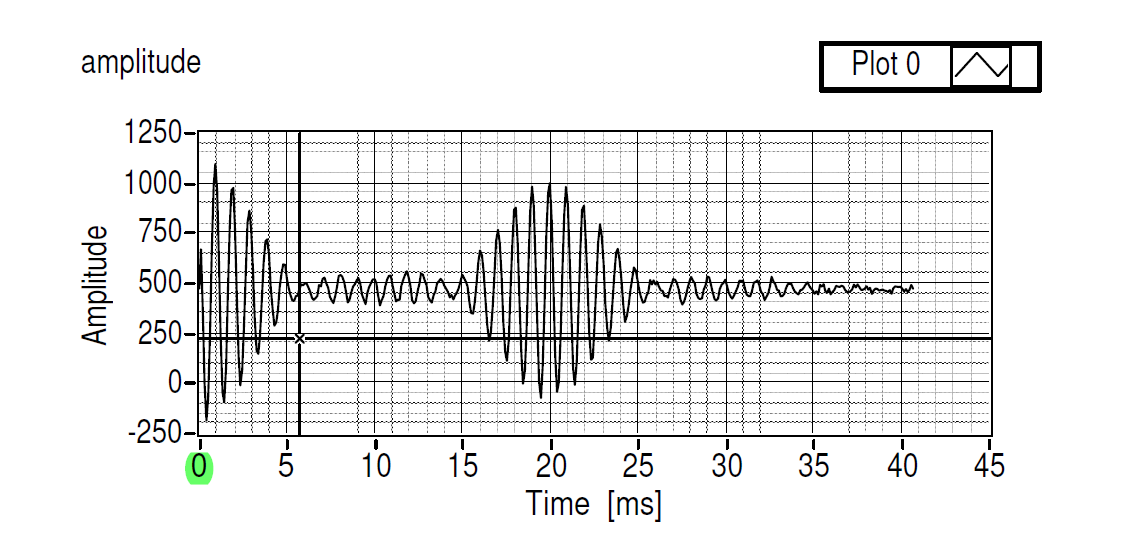
\includegraphics[width = .6\textwidth]{/Users/notchok/Documents/5. Semester/%FP/FP/F61/Latex images/spin_echo_signal.png}
%  \caption[]{Spin-echo by a 90-180 sequence  \footnotemark}
%    \label{fig: spin-echo signal}
% \end{center}
%\end{figure}
%\footnotetext{R. Schicker (2021, March 4). Nuclear Magnetic Resonance F61/F62 p. 13} 
Due to Parseval's theorem it is possible to estimate the signal's strength by calculating the area under the spin-echo curvature in frequency space.
%, which is given by a Gaussian profile. 
The decay curve of \ref{bloch + rot T2} is measured by varying the parameter $\tau$ in the 90°-180° sequence.

The Hahn echo finds its limitations when measuring the decay curvature for large $t$. In such cases the time evolution, due to the field inhomogenieties, is faster than the time scale of the measurement $\tau$, i.g the average Larmor frequencies in time intervals $0 < t < \tau$ and $\tau < t < 2 \tau$ can be different. Hence, only partial coherence can be achieved, leading to reduced signals and a reduced value for $T_2$.

\paragraph{Carr-Pulcell sequence: }
The Carr-Purcell methods consists of a 90° pulse that creates a transverse magnetization followed by repeated 180° pulses at odd multiples of $\tau$ that induce phase coherence at even multiples of $\tau$ as shown in Fig \ref{fig: carr-purcell sequence}. In this case $\tau$ is a small time interval. 
The sequence is repeated over a large interval of time yielding a value closer to the real value of the spin-spin relaxation time in comparison to the spin-echo method.
\begin{figure}[!htbp]
 \begin{center}
  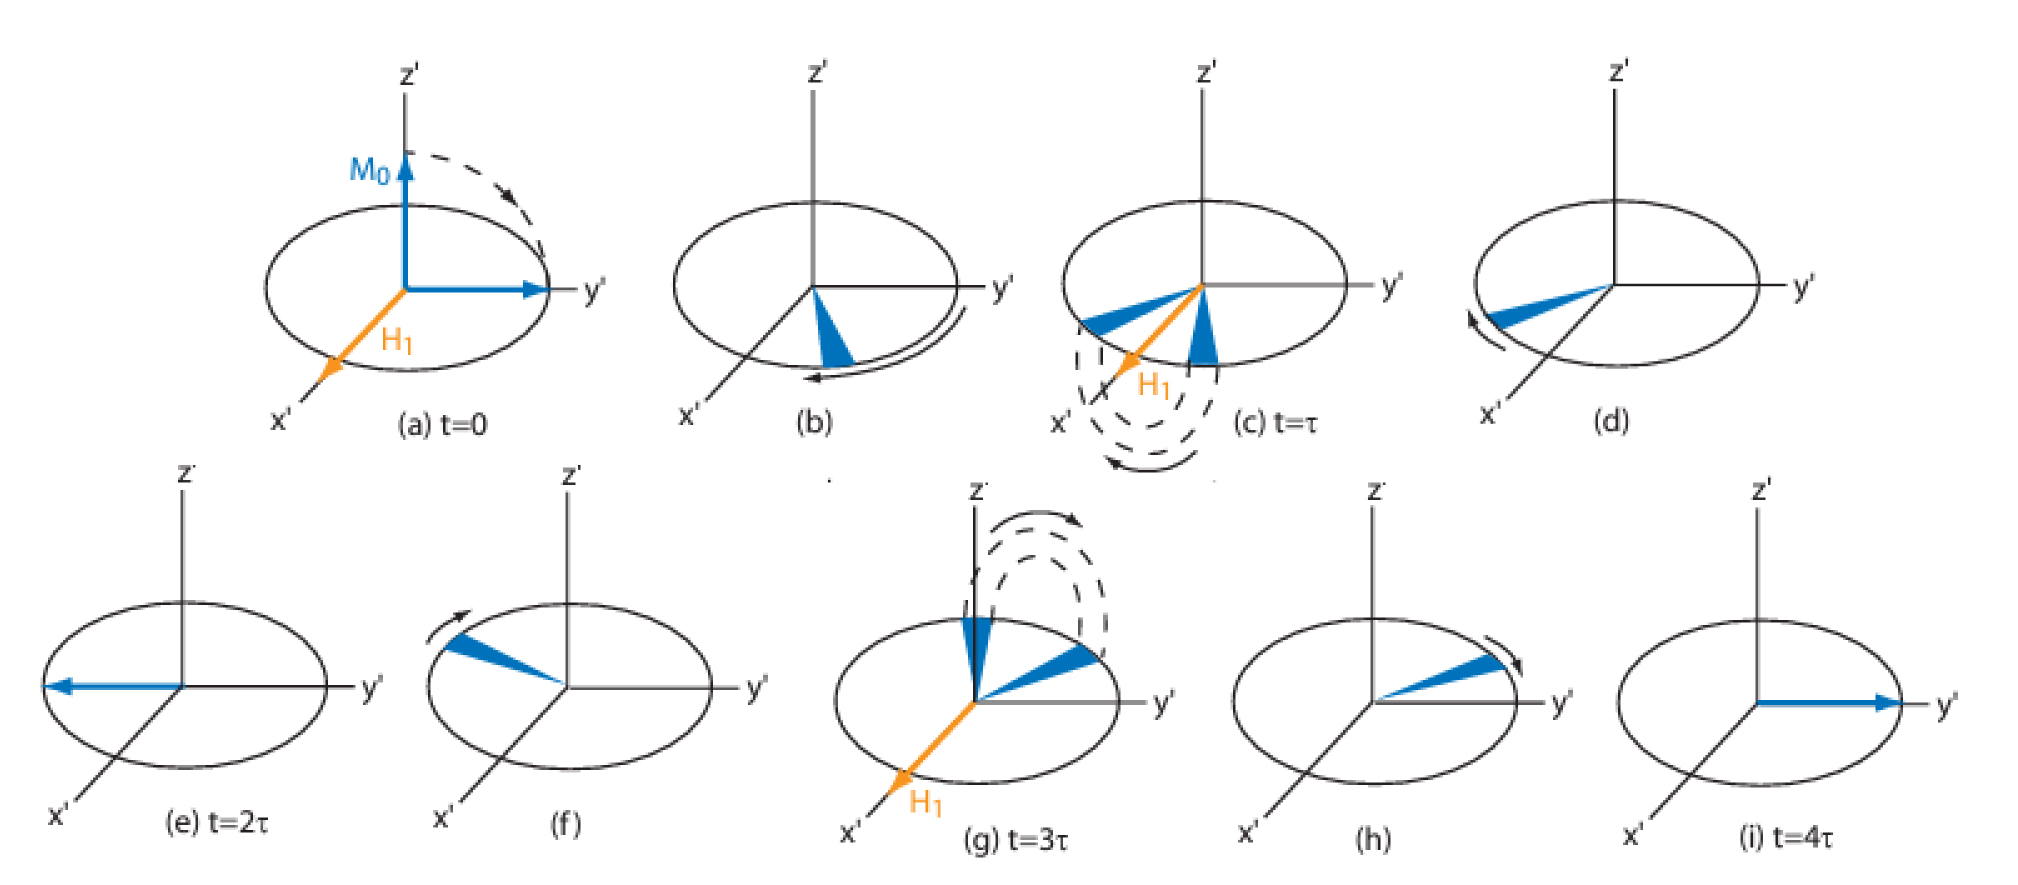
\includegraphics[width=.6\textwidth]{Latex images/carr-purcell-sequence2.jpg} 
  \caption[]{ Carr-Purcell sequence. a) 90° pulse, b) dephasing of magnetization, c) 180° pulse at $t = \tau$, d) rephasing e) spin-echo/ coherence at $t = 2\tau$, f) dephasing, g) 180° pulse at $t = 3 \tau$, h) rephasing, i) spin-echo at $t = 4\tau$.  \footnotemark}
  \label{fig: carr-purcell sequence}
 \end{center}
\end{figure}
\footnotetext{ (2013, March 13). Physikalisches Praktikum im Bachelor-Studiengangander RWTH Aachen Versuch:Nuclear Magnetic Resonance(NMR) p. 16 }

\subsubsection{Spin-lattice relaxation $T_1$}
An anti-parallel state will also decay by giving energy to its surroundings. This is the spin-lattice relaxation and it's described by  the solution of \ref{bloch + rot T1}:
\begin{equation}
\label{eq: sol. bloch T1}
\vec{M}_\parallel(t) = \vec{M}_0\left( 1 - 2e^{t/T_1}\right).
\end{equation}

After a 180° pulse a magnetization $\vec{M}_\parallel$ is generated, which is anti-parallel relative to the orientation of the field $B_0$. Since the an anti-parallel state doesn't produce a signal, a 90° pulse at $t = \tau$ is used to transform the magnetization into a transverse one. The signal at $t = \tau$ is proportional to the initial longitudinal state. The decay curve of $\vec{M}_\parallel$ can be measured by varying the value of $\tau$ in the pulse sequence 180°-90°. 
\subsection{Chemical shift}
Protons that are bounded to molecules do not interact with the external magnetic field alone, but rather with a field $\vec{B}_{tot}$ modified by the magnetic shielding of the electron orbitals. Hence, according to equation \ref{eq: larmor freq}, the Larmor frequency of the protons should be modified:
\begin{equation}
\omega_i = \omega_L\left( 1 - \sigma_i\right).
\end{equation}
Here $\omega_L$ is the free Larmor frequency, $\omega_i$ is the frequency modified by the chemical shift and $\sigma_i$ stands for the shielding factor, which is characterized by the molecule and each nucleus within the molecule.
In order to use this characteristic shielding factor to identify  the molecule Tetra-Methyl-Silan (TMS) was used as reference substance. Under this condition the chemical shift $\delta_i$ is given by:
\begin{equation}
\delta_i = \sigma_i - \sigma_{TMS} = \frac{\omega_{TMS} - \omega_i}{\omega_L}.
\end{equation}
\begin{figure}[!htbp]
 \begin{center}
  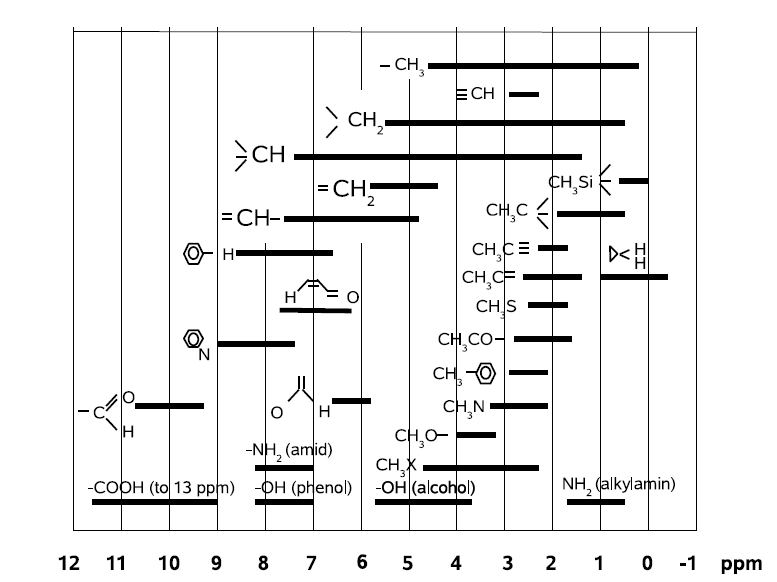
\includegraphics[width = .6\textwidth]{Latex images/chemical-shift.png}
  \caption[]{Chemical shift $\delta_i$ of differnt compounds relative to TMS \footnotemark}
    \label{fig: chemical shift}
 \end{center}
\end{figure}
\footnotetext{R. Schicker (2021, March 4). Nuclear Magnetic Resonance F61/F62 p. 19} 

s\subsection{Imaging with NMR}
The imaging measurements in the experiment were made with the Bruker NMR analyzer mq7.5. 
In order to carry out measurements, which contain information on the position of the produced NMR signal, position dependent fields are implemented. These fields are superimposed to the static field $\vec{B}_0$ which defines the z-axis. In the used set up all gradients are parallel to the static field and are linear functions of the corresponding coordinates:
$$\vec{B}^x = (0,0,G^x\cdot x)^T$$
$$\vec{B}^y = (0,0,G^y\cdot y)^T$$
$$\vec{B}^z = (0,0,G^z\cdot z)^T$$
\subsubsection{One dimensional imaging}
Let's consider the  1 dimensional imaging in z-direction, where only the $\vec{B}^z$ is used.  

Due to the field gradient the Larmor frequency becomes a linear function of position z:
\begin{equation}
\omega_L(z) = \gamma(B_0 + G^z\cdot z).
\end{equation}
After taking the rotating frame into consideration, where $\vec{M}_\perp$ is given by \ref{bloch + rot T2} and will be denoted as $\vec{M}_\perp^{rot}$, and the position dependent Larmor frequency we can write the transverse magnetization as:
\begin{equation}
\vec{M}_\perp(z, t) = M_\perp^{rot}(z,t)e^{i\gamma(B_0 + G^{z}z)t}.
\end{equation}
Using this expression one finds that the NMR signal is, apart from a phase factor, the Fourier transformation of the transverse magnetization $M_\perp^{rot}$:
\begin{equation}
S(t)\propto e^{i\Omega t} \int_{V} M_\perp^{rot}(z,t) e^{i\omega_z t} d\vec{x}.
\end{equation}
Hence $M_\perp^{rot(z)}$ can be deduced from the measured NMR signal $S(t)$ by a 1 dimensional Fourier transformation signal.

For the measurements there are two methods to generate the data points:
\paragraph{Frequency coding}
In this case the signal is measured as a function of time and we sample over $t_n = n\Delta t$ which gives a data set:
$$S_1 = S(\Delta t), \quad S_2 = S(2\Delta t), ..., S_N = S(N\Delta t)$$
\paragraph{Phase coding}
In this approach we use the fact, that during the readout the position information is related to the phase angle produced by the applied gradient:
\begin{equation}
\Delta \phi(z)= \phi(z)-\phi(0) = \gamma G^z z t= \omega_z t.
\end{equation}
Thus the gradient  $G^z$ is applied during a time interval $T_{Ph}$ before the read out, which induce a phase angle \begin{equation}
\phi(z) = (\gamma G^z T_{Ph})z = k_z z.
\end{equation}
Here $k_z$ is the position frequency. After this time the gradient is switched off. All the components of the magnetization precess with the original frequency but with different phase angles.  
To generated the data points the NMR signal is measured at a fixed time $t_0$ and sampled over different position frequencies $k_n = n\Delta k$ by varying the gradient strength in steps of $\Delta G^z$.  This results in the data set: 
$$S_1 = S(\Delta k_z,t_0), \quad S_2 = S(2\Delta k_z, t_0), ..., S_N = S(N\Delta k_z, t_0).$$

\subsubsection{Two dimensional imaging}
For two dimensional imaging we use a two dimensional Fourier method. In this case the measurement method consist in first choosing a slice $z_1 < z < z_2$ which will be selectively excited by a high frequency pulse of duration $t_p$. At this point the different positions in the slice have different Larmor frequencies due to the slice selection gradient. To generate a phase coherent system, a second high frequency pulse with opposite polarization of the duration $t_p/2$ is used. Consequently we implement a combination of phase coding in x-direction and frequency coding in y-direction to generate a matrix of $NxM$ data points $S(k_n, t_m)$. Finally the image can be derived by a two dimensional Fourier transformation. 













